\documentclass[a4paper 12pts]{article}
\usepackage[utf8]{inputenc}
\usepackage[T1]{fontenc}
\usepackage[francais]{babel}
\usepackage{graphicx}


\title{Documentation Technique : iRover}

\author{}

\begin{document}

\maketitle


\begin{figure}[h]
   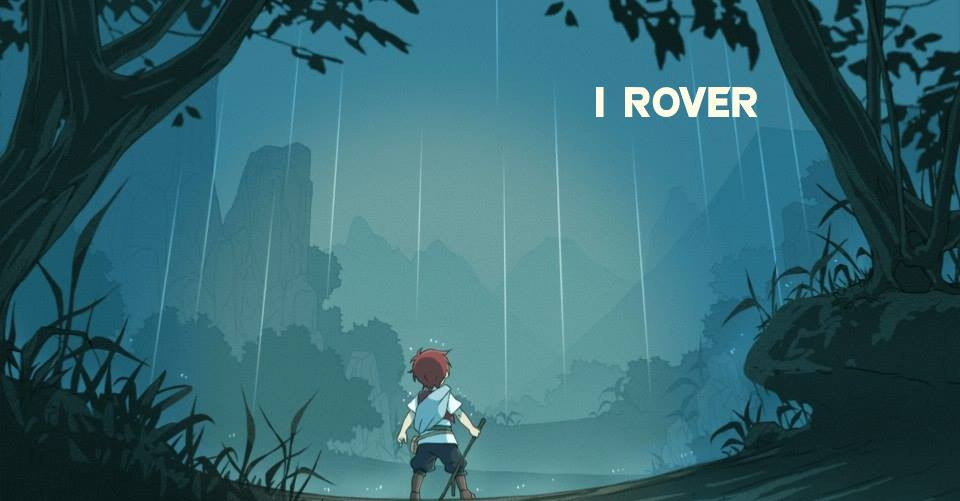
\includegraphics[width=350pt]{Illustration/proj_irover.jpg}
	\caption{iRover, l'histoire d'un héros qu'on appellait robot}
\end{figure}



\newpage


\renewcommand{\contentsname}{Sommaire} 
\tableofcontents

\newpage





\section{Manuel Documentation Technique}


\vspace{2cm}

Cette partie est dédiée aux développeur
%expliqué à quoi sert cette documentation


\section{Les personnages}

\subsection{Le robot, Rover}

\subsection{les ennemis}



\section{les coffres}

\section{les clé}


\section{L'environnement}


\section{La gestion des évênements}


\subsection {Rencontre avec un ennemi} 
\subsection {Ouvertude d'un coffre}
\subsection {Ramasser une clé}


\section{l'interface utilisateur}

\section{IA}

\subsection{path finding}

\subsection{découverte de la carte}

\section{condition fin de jeu}

\section {FAQ}




\end{document}

